% This file was created with tikzplotlib v0.10.1.
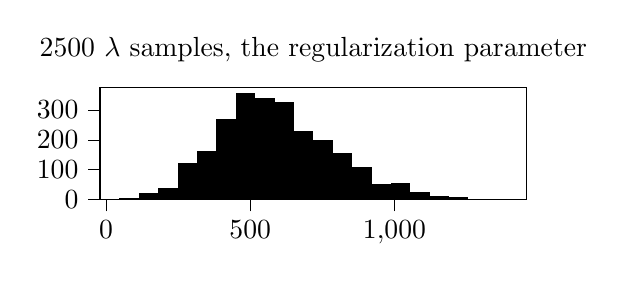
\begin{tikzpicture}

\definecolor{darkgray176}{RGB}{176,176,176}

\begin{axis}[
height=3cm,
tick align=outside,
tick pos=left,
title={2500 \(\displaystyle \lambda\) samples, the regularization parameter},
width=7cm,
x grid style={darkgray176},
xmin=-20.826318041018, xmax=1458.25119418142,
xtick style={color=black},
y grid style={darkgray176},
ymin=0, ymax=373.8,
ytick style={color=black}
]
\draw[draw=none,fill=black] (axis cs:46.404477969093,0) rectangle (axis cs:113.635273979204,6);
\draw[draw=none,fill=black] (axis cs:113.635273979204,0) rectangle (axis cs:180.866069989315,22);
\draw[draw=none,fill=black] (axis cs:180.866069989315,0) rectangle (axis cs:248.096865999426,40);
\draw[draw=none,fill=black] (axis cs:248.096865999426,0) rectangle (axis cs:315.327662009537,122);
\draw[draw=none,fill=black] (axis cs:315.327662009537,0) rectangle (axis cs:382.558458019648,164);
\draw[draw=none,fill=black] (axis cs:382.558458019648,0) rectangle (axis cs:449.789254029759,271);
\draw[draw=none,fill=black] (axis cs:449.789254029759,0) rectangle (axis cs:517.02005003987,356);
\draw[draw=none,fill=black] (axis cs:517.02005003987,0) rectangle (axis cs:584.250846049981,340);
\draw[draw=none,fill=black] (axis cs:584.250846049981,0) rectangle (axis cs:651.481642060092,327);
\draw[draw=none,fill=black] (axis cs:651.481642060092,0) rectangle (axis cs:718.712438070203,228);
\draw[draw=none,fill=black] (axis cs:718.712438070203,0) rectangle (axis cs:785.943234080314,200);
\draw[draw=none,fill=black] (axis cs:785.943234080314,0) rectangle (axis cs:853.174030090425,157);
\draw[draw=none,fill=black] (axis cs:853.174030090425,0) rectangle (axis cs:920.404826100536,109);
\draw[draw=none,fill=black] (axis cs:920.404826100536,0) rectangle (axis cs:987.635622110647,53);
\draw[draw=none,fill=black] (axis cs:987.635622110647,0) rectangle (axis cs:1054.86641812076,56);
\draw[draw=none,fill=black] (axis cs:1054.86641812076,0) rectangle (axis cs:1122.09721413087,25);
\draw[draw=none,fill=black] (axis cs:1122.09721413087,0) rectangle (axis cs:1189.32801014098,11);
\draw[draw=none,fill=black] (axis cs:1189.32801014098,0) rectangle (axis cs:1256.55880615109,7);
\draw[draw=none,fill=black] (axis cs:1256.55880615109,0) rectangle (axis cs:1323.7896021612,3);
\draw[draw=none,fill=black] (axis cs:1323.7896021612,0) rectangle (axis cs:1391.02039817131,3);
\end{axis}

\end{tikzpicture}
